
\chapter{Lecture Allocation}

\section{Introduction}

The goal of the lecture allocation problem is to allocate course lectures to faculty members in a way that ensures the students have a good learning experience and the faculty members are not overworked. The previous chapter identified the amount of workload that each faculty member can handle. In this chapter, the lecture allocation process is designed to incorporate this workload limit, along with the student feedback for the faculty members.

Additionally, it will also incorporate the faculty preference towards certain courses, and the management priority of ensuring that the earlier-year courses are taught by the best faculty members, all while ensuring that the lectures are allocated equitably among the faculty members.

The lecture allocation problem will be defined and modeled as a multi-constraint optimization problem which will be solved using the Hungarian algorithm. The course-faculty fit metric will be defined to represent the suitability of a faculty member to teach a course, which will be used by the Hungarian algorithm.

Additional constraints will be added to the technique to honor the workload limits of the faculty, and additional techniques will be introduced to ensure the allocation of all course lectures without exceeding these workload limits.

In the following sections, these techniques will be discussed in detail and the experimental results of the lecture allocation process applied to real-world data will be analyzed.

\section{Factors affecting Course-Faculty Fit}

The first step towards solving the allocation problem is defining what makes a faculty member suitable to teach a course. This should incorporate the priorities of the students, the management, and the faculty members. Additionally, it should also be easy to understand and explain, easy to collect the data required to compute it, and easy to compute. It should also be easy to tweak and improve, since the priorities of different institutions may be different.

\subsection{Student Feedback}

The students are the most important stakeholders in the decision of which faculty member should teach a course since their learning experience and outcomes are directly affected by this decision. Their priorities are to be taught by a faculty member who is experienced at teaching and knowledgeable about the subject matter. This priority can be quantified by collecting the feedback of the students about the faculty member who taught the course in the past.

At the end of a semester, the student feedback is collected on their learning experience in the courses they were taught. This feedback is collected in the form of a survey, which is filled out by the students and submitted to the management. The survey contains questions about the faculty members who taught the course, the course content, the pace of the course, and the overall learning experience. The feedback is collected for each course and faculty member combination. This feedback may also be collected periodically during the semester, especially for courses that are taught in multiple parts by different faculty members.

Peer feedback collected from the faculty members of the department can also be used to evaluate the teaching performance of the faculty members. This includes questions about the teaching performance of the faculty members and their knowledge of the subject matter.

These feedback components are then combined into a \textbf{Student Feedback Score} for each course-faculty combination, which is a number between 0 to 5. This score is calculated by taking a weighted average of the student feedback and the peer feedback, with student feedback being weighted more than the peer feedback since the student feedback is more representative of the learning experience of the students.

Since there are also faculty who are eligible to teach a course but have never taught the course before, they will not have any student feedback. In this case, the peer feedback is combined with the average student feedback for the course to calculate the Student Feedback Score.

\subsection{Faculty Preference and Expertise}

With manual allocation, faculty members are often left with courses they prefer not to teach. The largely static allocation process leaves faculty members with similar teaching assignments every semester, which may lead to a lack of motivation and interest in teaching. With the automated allocation process, faculty members will be considered to teach courses that they are interested in, which will lead to a better learning experience for the students and a better teaching experience for the faculty members.

Before every semester, the faculty are asked to submit their preferences for the courses they would like to teach. This is done by asking the faculty members to rank the courses they are eligible to teach in the order of their preference. They are required to rank every course that they are eligible to teach, which also forms the basis for the course-eligibility criteria since they should not be given courses that are completely out of their area of expertise. Additionally, the courses they have taught in the past are also treated as eligible courses, even if they are not directly ranked by the faculty. The management requires the faculty to provide a minimum number of preferences to ensure that courses are not left unallocated.

These preference scores are then normalized to a number between 0 to 5 to form the \textbf{Faculty Preference Score} for each course-faculty combination. This score is calculated by taking the list of preferences provided by the faculty and linearly distributing it between 0 to 5, such that the first preference is given a score of 5, and the tenth preference is given a score of 0. The preferences for courses beyond the tenth preference are given a score of 0. The courses that are not ranked by the faculty are also given a score of 0.

\subsection{Management Priorities}

The management priority is to ensure the long-term learning path of the students is optimal throughout the program. This means establishing a strong foundation for the students in the early years of their program and then building on that foundation in the later years. This is done by ensuring that the course lectures in the early years of the degree are taught by highly experienced faculty members with good teaching performance scores. The latter-year course lectures on the other hand can be allocated with a higher priority to the faculty members who are more interested in teaching the course since this is reflective of the faculty's research interests, which makes them more knowledgeable about the subject matter for the advanced courses in the program.

This can be achieved by ensuring that the higher-year courses are given priority to be taught by the faculty members with the best ratings. This prioritization is done in an absolute manner, where the courses are allocated in the sequence of their year of study, thus ensuring that the courses in the earlier years can reserve the best faculty members. This will be discussed in detail in the next section.

\section{Modelling Lecture Allocation Problem}

The lecture allocation problem can be modeled as an assignment problem, where the tasks are the lectures of each course, and the agents are the faculty members who are teaching the course. Each lecture's assignment to a faculty member should have a cost that represents the objectives of the allocation problem. Every lecture of a course must be assigned to exactly one faculty member, while each faculty member may be assigned to multiple lectures of multiple courses.

The cost of assigning a course to a faculty member should represent the suitability of the faculty member to teach the course by taking into account student feedback. It should also represent the preference of the faculty member to teach the course by using the faculty preference rankings provided by the faculty members. Additionally, the allocation of low-cost faculty members to earlier-year courses should be prioritized to ensure that the earlier-year courses are taught by the best faculty members.

It also needs to be ensured that the workload is distributed among the faculty members in proportion to their relative teaching workload, which was defined in the previous chapter. This proportionality is achieved by ensuring that the workload of the faculty members does not exceed their workload limits, where the workload limits are defined as proportional to the faculty's relative teaching workload.

In the next section, we will define how this constrained cost-minimization problem can be solved using the Hungarian algorithm.

\subsection{Hungarian Algorithm for Optimal Allocation}

The Hungarian Algorithm, also known as the Kuhn-Munkres Algorithm, is a combinatorial optimization algorithm that solves the assignment problem in polynomial time. In comparison to other algorithms that solve the assignment problem, such as the genetic algorithm and the simulated annealing algorithm, the Hungarian algorithm is faster, more efficient, and more deterministic. This makes it a good choice for solving the lecture allocation problem since the faculty, students, and management expect the allocation to be deterministic.

The Hungarian algorithm solves the assignment problem by finding the optimal assignment between the tasks and the agents, where each task is assigned to exactly one agent, and each agent is assigned to exactly one task. The optimal assignment is the one that minimizes the total cost of assigning the tasks to the agents. For an unequal number of tasks and agents, the Hungarian algorithm can be used to find the optimal assignment by adding dummy tasks or dummy agents, which are assigned a cost of 0. This ensures that the total cost of the assignment is not affected by the dummy tasks or dummy agents. This also means that for more tasks than agents, some of the tasks will be left unassigned.

However, a university typically has more lectures than the number of faculty members, which means that each faculty member will have to teach multiple lectures of a course. Thus, the allocation problem is split into multiple iterations of the Hungarian algorithm, where each iteration allocates one lecture of each course to a faculty member.

The cost matrix for the Hungarian algorithm is constructed by calculating the cost of assigning each course to each faculty member. The cost of assigning a course to a faculty member is calculated by taking the course-faculty fit metric and subtracting it from 5. This is done to ensure that the cost of assigning a course to a faculty member is inversely proportional to the course-faculty fit metric since the Hungarian algorithm minimizes the total cost of the assignment. The cost matrix is constructed using the algorithm shown in \autoref{alg:cost_matrix_construction}.

\begin{algorithm}[H]
  \caption{Cost Matrix Construction for Lecture Allocation}
  \begin{algorithmic}[1]
    \Procedure{ConstructMatrix}{$lectures$, $faculty$}
    \For{$l \in lectures$}
    \For{$f \in faculty$}
    \If{$f \text{ can teach } l$}
    \State $cost \gets Q(l, f)$
    \Else
    \State $cost \gets \infty$
    \EndIf
    \State $costMatrix[l][f] \gets cost$
    \EndFor
    \EndFor
    \EndProcedure
  \end{algorithmic}
  \label{alg:cost_matrix_construction}
\end{algorithm}

where, \(lectures\) is the list of lectures of each course, \(faculty\) is the list of faculty members, and \(Q(l, f)\) is the cost function for assigning course lecture \(l\) to faculty member \(f\).

With the cost matrix constructed, the Hungarian algorithm can be used to allocate the lectures of each course to the faculty members who are teaching the course. The allocation process is split into multiple iterations of the Hungarian algorithm, where each iteration allocates one lecture of each course to a faculty member.

In each iteration of the loop, we use \autoref{alg:cost_matrix_construction} to construct the cost matrix, and then use the Hungarian algorithm to find the optimal assignment between the courses and the faculty members. Some of these assignments may be dummy assignments that are created due to the unequal number of courses and faculty members. These dummy assignments are ignored, and the remaining assignments are added to the list of all assignments. We run this loop until all the lectures are allocated. However, if no new lectures are allocated in an iteration, then the loop is broken since no progress is being made. This is shown in \autoref{alg:base_lec_alloc}.

\begin{algorithm}[H]
  \caption{Lecture Allocation Algorithm}
  \begin{algorithmic}[1]
    \Procedure{AllocateLectures}{$lectures$, $faculty$}
    \State $unallocatedLectures \gets lectures$
    \State $allocatedLectures \gets \emptyset$
    \State $allAssignments \gets \emptyset$
    \While {$unallocatedLectures \neq \emptyset$} \Comment{Iterate until all lectures are allocated}
    \State $costMatrix \gets \text{ConstructMatrix}(unallocatedLectures, faculty)$
    \State $assignments \gets \text{HungarianAlgorithm}(costMatrix)$
    \State $assignedCount \gets 0$
    \For {$assignment \in assignments$}
    \If {$assignment \text{ is not a dummy assignment}$}
    \State $allAssignments \gets allAssignments \cup assignment$
    \State $allocatedLectures \gets allocatedLectures \cup assignment$
    \State $unallocatedLectures \gets unallocatedLectures \setminus assignment$
    \State $assignedCount \gets assignedCount + 1$
    \EndIf
    \EndFor
    \If {$assignedCount = 0$}
    \State \textbf{Break Loop}
    \Comment{if no new lectures allocated, break the loop}
    \EndIf
    \EndWhile
    \State \Return $allAssignments$
    \EndProcedure
  \end{algorithmic}
  \label{alg:base_lec_alloc}
\end{algorithm}

where, \(lectures\) is the list of lectures of each course, \(faculty\) is the list of faculty members, \(unallocatedLectures\) is the list of lectures that are yet to be allocated, \(allocatedLectures\) is the list of lectures that are already allocated, and \(allAssignments\) is the list of all the assignments made by the Hungarian algorithm.

This lecture allocation algorithm $AllocateLectures$ forms the basis for the lecture allocation process in the latter stages, and is used as the building block for the various strategies proposed in the following sections. It involves multiple iterations of the Hungarian algorithm, where each iteration allocates one lecture of each course to a faculty member.

The Hungarian algorithm is run in each iteration until all the lectures are allocated. The assignments made by the Hungarian algorithm are then added to the list of all assignments, and the allocated lectures are removed from the list of unallocated lectures. This process is repeated until all the lectures are allocated.

\section{Lecture Allocation Objectives}
\label{sec:defining_the_allocation_problem}

The lecture allocation involves allocating the lectures of each course to the faculty members who are eligible to teach the course. It can be defined as a constrained multi-objective optimization problem, with a set of objectives that need to be optimized and a set of constraints that need to be satisfied.

The primary objective of the allocation problem is to ensure that all the courses are allocated to the faculty members since unallocated courses will lead to the cancellation of the course. Additionally, the allocation problem should also ensure that the workload of the faculty members is distributed equitably and that they receive a similar workload in terms of lectures, tutorials, and practicals. The allocation problem should also ensure that the earlier-year courses are taught by the best faculty as per the management priorities. Finally, the allocation problem should ensure that the faculty members are allocated the courses that they are interested in teaching, which will lead to a better teaching experience for the faculty members. These objectives are described in detail in the following sections, in the order of their priority.

\begin{enumerate}
  \item \textbf{Allocation of all lectures}

        The allocation problem should ensure that all the lectures are allocated to a faculty member. This is a hard constraint of the allocation problem since unallocated lectures will lead to cancellation of the course, which will adversely impact the learning experience of the students, and may impact their long-term learning path since some lectures may form a prerequisite for other courses.

        There are some prerequisites to this constraint - the allocation process cannot allocate a course if there are no eligible faculty members to teach the course, or if the maximum workload for the faculty members is already reached. However, given that these prerequisites are met, the allocation process should ensure that all the courses are allocated.

  \item \textbf{Proportionate distribution of teaching workload}

        The relative teaching workload, defined in the previous chapter, is a measure of the amount of teaching workload that a faculty member can handle, relative to the other faculty members. Thus, distributing the workload in proportion to the relative teaching workload ensures that the teaching workload is distributed equitably among the faculty members, ensuring that no faculty member is overworked.

  \item \textbf{Proportionate distribution of lectures, tutorials, and practicals to each faculty member}

        A course consists of multiple teaching activities, such as lectures, tutorials, and practicals. Preferably, these teaching activities should be distributed equally among the faculty members, so that each faculty member has a similar teaching experience. This is a soft constraint of the allocation problem since it is not as important as the other objectives, but it is still desirable to have a balanced teaching experience for the faculty members.

  \item \textbf{Preferential allocation of earlier-year courses}

        The management priority is to ensure that the earlier-year courses are taught by the faculty members with the best ratings since this is the foundation for the learning path of the students. This means that the earlier-year courses should be allocated with a higher priority to the faculty members with the best ratings. This is a soft constraint of the allocation problem since it is not as important as the other objectives, but it is still desirable to have the earlier-year courses taught by the best faculty members.

  \item \textbf{Maximizing faculty performance score}

        The faculty performance score, defined in the previous section, is a measure of the suitability of a faculty member to teach a course. It is representative of the student learning experience, and thus, maximizing the total faculty performance score of the allocation ensures that the students have a good learning experience. This is the primary objective of the allocation problem.

  \item \textbf{Maximizing faculty preference score}

        The faculty preference score, defined in the previous section, is a measure of the preference of the faculty member to teach a course. Thus, maximizing the total faculty preference score of the allocation ensures that the faculty members are allocated the courses that they are interested in teaching, which will lead to a better teaching experience for the faculty members.

        This is treated as a secondary objective of the allocation problem since it is not as important as the primary objective of maximizing the faculty performance score. However, given that the faculty performance score is comparable between the two allocations, the allocation with the higher faculty preference score is preferred.

\end{enumerate}

\subsection{Enforcing Workload Limits}

With the lecture allocation algorithm defined in \autoref{alg:base_lec_alloc}, the lectures of each course are allocated to the faculty members who are teaching the course. However, this allocation does not take into account the existing workload of the faculty members, which may lead to a disproportionate allocation of workload. To counter this, the allocation algorithm is modified to enforce the workload limits of the faculty members.

To enforce the workload limits, we first define the workload limits of the faculty members using the relative teaching workload, which was defined in the previous chapter. Then we incorporate the workload limits into the lecture allocation algorithm by modifying the cost matrix construction algorithm to ensure that the workload of the faculty members does not exceed their workload limits.

\subsubsection{Defining the Workload Limits}

The workload limits of the faculty members are previously defined in \autoref{sec:determining_equitable_teaching_workload} as the relative teaching workload. The relative teaching workload is a measure of the amount of teaching workload that a faculty member can handle, relative to the other faculty members. However, the workload of the faculty members is defined in terms of workload units, while the workload limits are defined relative to the other faculty members. Thus, the workload limits need to be converted to workload units to be enforced.

To convert the workload limits to workload units, the total workload units of the department are calculated, which is the sum of the workload units of all the courses. The workload limits of the faculty members are then converted to workload units by multiplying the workload limits with the total workload units of the department and dividing them by the total number of relative workload units of the faculty members. This is shown in \autoref{eq:workload_limits}.

\begin{equation}
  \label{eq:workload_limits}
  \begin{aligned}
    T_{total} & = \sum_{c \in courses} T_c               \\
    R_{total} & = \sum_{f \in faculty} R_f               \\
    T_f       & = R_f \times \frac{T_{total}}{R_{total}}
  \end{aligned}
\end{equation}

where,
\begin{align*}
  T_{total} & = \text{Total workload units of the department}               \\
  T_c       & = \text{Workload units of the course } c                      \\
  R_{total} & = \text{Total relative workload units of the faculty members} \\
  R_f       & = \text{Relative workload units of the faculty member } f     \\
  T_f       & = \text{Workload units limit of the faculty member } f
\end{align*}

\subsubsection{Lecture Allocation with Workload Limits}

With the workload limits of the faculty members defined in terms of workload units, the lecture allocation algorithm is modified to enforce the workload limits of the faculty members. This is done by ensuring that the workload of the faculty members does not exceed their workload limits at the time of cost matrix construction. This is shown in \autoref{alg:workload_limit_cost_matrix_construction}.

\begin{algorithm}[H]
  \caption{Cost Matrix Construction with Workload Limits}
  \begin{algorithmic}[1]
    \Procedure{ConstructMatrixWithWorkloadLimits}{}
    \For{$l \in lectures$}
    \For{$f \in faculty$}
    \If{($f \text{ can teach } l) \text{ and } (existingWorkload[f] + T[l]$ \textless $workloadLimits[f]$)}
    \State $cost \gets 5 - Q(l, f)$
    \Else
    \State $cost \gets \infty$
    \EndIf
    \State $costMatrix[l][f] \gets cost$
    \EndFor
    \EndFor
    \Return $costMatrix$
    \EndProcedure
  \end{algorithmic}
  \label{alg:workload_limit_cost_matrix_construction}
\end{algorithm}

where, \(lectures\) is the list of lectures of each course, \(faculty\) is the list of faculty members, \(existingWorkload\) is the already allocated workload of the faculty members, \(T[l]\) is the workload units of the lecture \(l\), and \(workloadLimits\) is the workload limits of the faculty members.

By using this modified cost matrix construction algorithm, the workload limits of the faculty members are enforced every time the Hungarian algorithm is run. This ensures that the workload of the faculty members are ineligible to teach a course if their workload exceeds their workload limits.

\subsection{Incorporating Management Priority}

The management priority is to ensure that the earlier-year courses are taught by the faculty members with the best ratings since this is the foundation for the learning path of the students. This means that the earlier-year courses should be allocated with a higher priority to the faculty members with the best ratings.

Since the faculty has a finite workload limit, as defined in the previous section, the faculty members with the best ratings have to be allocated to the earlier-year courses first, since the courses that are allocated first might fulfill the workload limits of the faculty members, thus making them ineligible to teach any courses that are allocated later. This is especially true for the faculty members with a low workload limit since they can only teach a few courses, and thus, they have to be allocated to the earlier-year courses first.

To achieve this, the courses are allocated in the sequence of their year of study, thus ensuring that the courses in the earlier years can reserve the best faculty members. This is done by iterating over the courses in the order of their year of study and allocating the courses in that order. This ensures that the courses in the earlier years are allocated first, and thus, they can reserve the best faculty members, meeting the hard constraint of the management priority.

The lecture allocation algorithm is modified to incorporate this approach by filtering the list of courses to be allocated by the year of study, then iterating over the filtered list of courses year-wise, and allocating the courses in that order. This is shown in \autoref{alg:year_wise_lec_alloc}.

\begin{algorithm}[H]
  \caption{Year-wise Lecture Allocation Algorithm}
  \begin{algorithmic}[1]
    \Procedure{AllocateLecturesYearwise}{$lectures$, $faculty$}
    \State $allAssignments \gets \emptyset$
    \For{$year \gets 1$ to $maxYear$} \Comment{Iterate over the years}
    \State $yearLectures \gets \text{FilterByYear}(lectures, year)$
    \State $yearAllocations \gets AllocateLecturesWithWorkloadLimits(yearLectures, faculty)$
    \State $allAssignments \gets allAssignments \cup yearAllocations$
    \EndFor
    \State \Return $allAssignments$
    \EndProcedure
  \end{algorithmic}
  \label{alg:year_wise_lec_alloc}
\end{algorithm}

where, $AllocateLecturesWithWorkloadLimits$ is the lecture allocation algorithm defined in \autoref{alg:base_lec_alloc}, but using the cost matrix construction algorithm that uses the faculty workload limits, as defined in \autoref{alg:workload_limit_cost_matrix_construction}.

% \subsection{Soft Priority}

% In this approach, the courses are allocated in a soft manner, biasing the allocation of earlier-year courses towards the best faculty members by manipulating the course-faculty fit metric. This is done by reducing the cost of assigning a course to well-rated faculty members and increasing the cost of low-rated faculty members in earlier-years courses.

% This bias factor that is introduced in the course-faculty fit metric is kept as a configurable parameter, which is higher for the earlier-year courses and lower for the later-year courses. This ensures that the earlier-year courses are allocated with a higher priority to the faculty members with the best ratings, while the later-year courses are allocated with a lower priority to the faculty members with the best ratings. The biases used for the different years are shown in Table \autoref{tab:year_wise_bias}.

% \begin{table}[H]
%   \centering
%   \begin{tabular}{|c|c|c|c|c|c|}
%     \hline
%     \textbf{Year} & \textbf{1} & \textbf{2} & \textbf{3} & \textbf{4} & \textbf{5} \\ \hline
%     \textbf{Bias} & 1          & 0.75       & 0.5        & 0.25       & 0          \\ \hline
%   \end{tabular}
%   \caption{Year-wise Bias}
%   \label{tab:year_wise_bias}
% \end{table}

% Additionally, the best faculty members need to be defined, which is done by defining a threshold Teaching Performance Score. The faculty members with a Teaching Performance Score above the threshold are considered to be the best faculty members. This threshold is kept as a configurable parameter, which can be tweaked to suit the priorities of the institution. As a default, the threshold Teaching Performance Score is kept at 4.5, which filters out the top-performing faculty members from the rest.

% With the biases and the threshold Teaching Performance Score defined, the cost matrix calculation algorithm is modified to incorporate the soft priority approach. This is shown in \autoref{alg:soft_priority_cost_matrix_construction}.

% \begin{algorithm}[H]
%   \caption{Soft Priority: Biased Cost Matrix Construction}
%   \begin{algorithmic}[1]
%     \Procedure{ConstructBiasMatrix}{$lectures$, $faculty$}
%     \For{$l \in lectures$}
%     \For{$f \in faculty$}
%     \If{$f \text{ can teach } l$}
%     \State $fitScore \gets Q(l, f)$
%     \If{$fitScore \geq threshold$} \Comment{if faculty is one of the best faculty members}
%     % sum of cost and bias
%     \State $cost \gets cost - getBias(l.year)$
%     \Else
%     \State $cost \gets cost + getBias(l.year)$
%     \EndIf
%     \Else
%     \State $cost \gets \infty$
%     \EndIf
%     \State $costMatrix[l][f] \gets cost$
%     \EndFor
%     \EndFor
%     \EndProcedure
%   \end{algorithmic}
%   \label{alg:soft_priority_cost_matrix_construction}
% \end{algorithm}

\subsection{Defining the Cost Function (\texorpdfstring{$Q$}{Q})}
\label{sec:defining_the_cost_function}

To solve the lecture allocation problem using the Hungarian algorithm, a cost function \(Q\) needs to be defined, which represents the suitability of a faculty member to teach a course. This cost function is used to calculate the cost of assigning a course to a faculty member, which is used by the Hungarian algorithm to find the optimal assignment between the courses and the faculty members.

To define the cost function, we first define a course-faculty fit metric. This course-faculty fit metric is a number between 0 to 5 that represents the suitability of a faculty member to teach a course. This metric is calculated by taking a weighted average of the Student Feedback Score and the Faculty Preference Score, with the Student Feedback Score being weighted more than the Faculty Preference Score. This is done to ensure that the student priorities are given more weightage than the faculty priorities. The Student Feedback Score and the Faculty Preference Score are weighted by a factor of 9 and 1 respectively.

\begin{equation}
  \label{eq:course_faculty_fit}
  \begin{aligned}
    FitScore = \frac{9 \times \text{Feedback} + 1 \times \text{Pref}}{10}
  \end{aligned}
\end{equation}

where, \textbf{Feedback} is the Student Feedback Score and \textbf{Pref} is the Faculty Preference Score, both of which have a range of 0 to 5. \(FitScore\), \textbf{Perform} and \textbf{Pref} are all calculated and evaluated for each course-faculty combination separately.

The course faculty fit metric is used to define the cost function of the Hungarian algorithm, which is to maximize the sum of the course-faculty fit metric of all the allocated courses. This ensures that the courses are allocated to the faculty members who are most suitable to teach them, thus ensuring a good learning experience for the students and a good teaching experience for the faculty members.

It is important to note that the course-faculty fit metric is configurable and can be tweaked to suit the priorities of the institution. For example, if the institution prioritizes the faculty preferences over the student priorities, the Teaching Performance Score can be weighted less than the Faculty Preference Score. This can be done by changing the weightage of the Teaching Performance Score and the Faculty Preference Score in \autoref{eq:course_faculty_fit}

\subsection{Experimental Results}

The lecture allocation algorithm uses the Hungarian algorithm to allocate the lectures of each course to the faculty members who are teaching the course. The Hungarian algorithm is run in each iteration until all the lectures are allocated. The cost function for the Hungarian algorithm is defined in \autoref{sec:defining_the_cost_function}, which is used to calculate the cost matrix for the Hungarian algorithm. In this cost matrix construction, the workload limits of the faculty members are enforced to ensure that the workload of the faculty members does not exceed their workload limits. Additionally, the courses are allocated in the sequence of their year of study, thus ensuring that the courses in the earlier years can reserve the best faculty members.

Using this approach, the lecture allocation algorithm was run on the dataset of the School of Computer Science and Engineering, Nanyang Technological University, Singapore. The results of this allocation are shown in \autoref{tab:lec_alloc_results}.

\begin{table}[H]
  \centering
  \begin{tabular}{|l|c|c|c|c|c|r|}
    \hline
    \textbf{Year} & \textbf{1} & \textbf{2} & \textbf{3} & \textbf{4} & \textbf{5} & \textbf{Total} \\ \hline
    Assigned      & 32         & 23         & 12         & 6          & 2          & 75             \\ \hline
    Unassigned    & 8          & 8          & 12         & 20         & 12         & 60             \\ \hline
    Avg Score     & 3.62       & 3.71       & 3.44       & 3.43       & 3.75       & 3.60           \\ \hline
  \end{tabular}
  \caption{Lecture Allocation Results}
  \label{tab:lec_alloc_results}
\end{table}

As visible in the results, there are 60 unallocated lectures, which is 44\% of the total lectures. This is partially because the courses in the earlier years are allocated first, which means that certain faculty members may reach their workload limits before the courses in the later years are allocated. However, this is also because there is an inherent asymmetry in the demand and supply of faculty members, i.e. the faculty in high demand may or may not be in high supply, and vice versa. This is discussed in detail in the next section.

\begin{figure}[H]
  \centering
  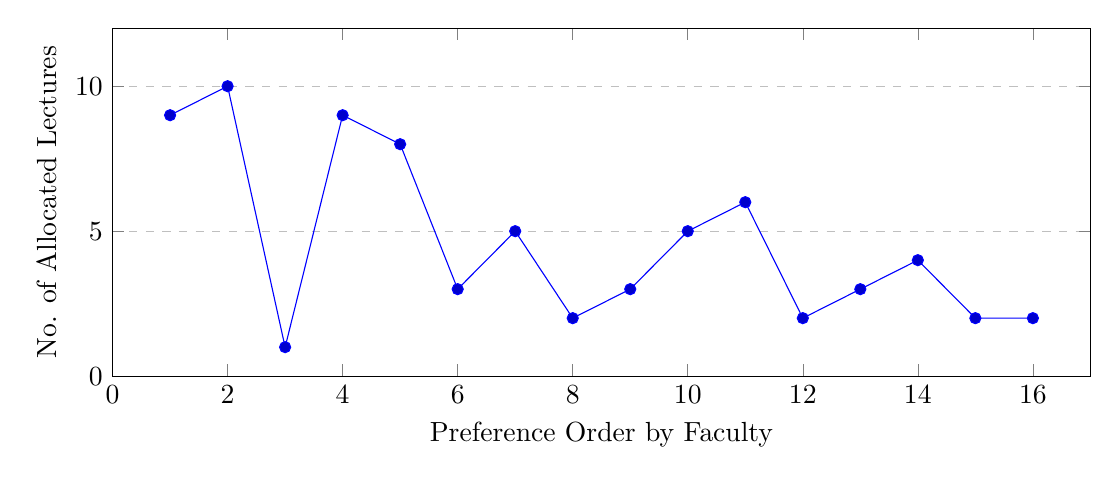
\begin{tikzpicture}
    \begin{axis}[
        xlabel={Preference Order by Faculty},
        ylabel={No. of Allocated Lectures},
        xmin=0, xmax=17,
        ymin=0,
        ymax=12,
        width=14cm,
        height=6cm,
        legend style={at={(0.5,-0.15)},
            anchor=north,legend columns=-1},
        ymajorgrids=true,
        grid style=dashed
      ]
      \addplot coordinates {
          (1, 9)
          (2, 10)
          (3, 1)
          (4, 9)
          (5, 8)
          (6, 3)
          (7, 5)
          (8, 2)
          (9, 3)
          (10, 5)
          (11, 6)
          (12, 2)
          (13, 3)
          (14, 4)
          (15, 2)
          (16, 2)
        } ;
    \end{axis}
  \end{tikzpicture}
  \caption{Allocation of Lectures by Faculty Preference Order}
  \label{fig:pref_order}
\end{figure}

\autoref{fig:pref_order} shows how the preference order of the faculty members impacts the allocation. As visible in the figure, the faculty members with a low preference order are allocated more lectures than the faculty members with a high preference order. This shows the effectiveness of the cost function based on the course-faculty fit (\autoref{eq:course_faculty_fit}), which takes into account the faculty preference score while allocating the lectures.

\section{Techniques for Resolving Unallocated Courses}
\label{sec:rectifying_unallocated_courses}

With the allocation approach defined so far, certain courses remain unallocated due to the year-wise prioritization of courses and the workload limits of the faculty. These issues are caused by the fact that the courses in the earlier years are allocated first, which means that certain faculty members may reach their workload limits before the courses in the later years are allocated. However, allocating all the courses is a definite requirement of the allocation problem, which means that the courses in the later years have to be accounted for in the allocation process.

\autoref{fig:faculty_utilization} shows the utilization of the faculty members, i.e. the workload allocated to the faculty members as a percentage of their workload limits. The figure shows that there are 47 faculty members with a utilization of 0, which means that they are not allocated any lectures. This is partially due to the demand and supply asymmetry, but also because some lectures might have a workload too high for a single faculty member to handle, which means that multiple faculty members have to be allocated to the lecture.

\begin{figure}[H]
  \centering
  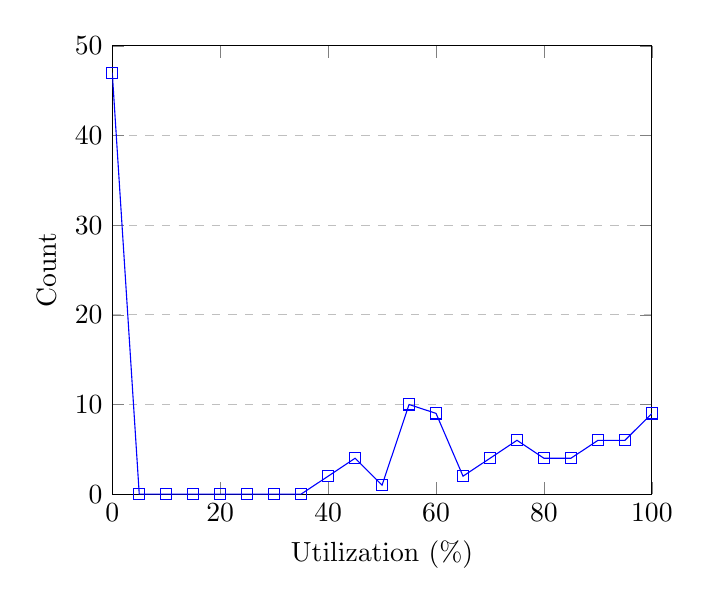
\begin{tikzpicture}
    \begin{axis}[
        xlabel={Utilization (\%)},
        ylabel={Count},
        xmin=0, xmax=100,
        ymin=0, ymax=50,
        xshift=0.5cm,
        legend pos=north west,
        ymajorgrids=true,
        grid style=dashed,
      ]

      \addplot[
        color=blue,
        mark=square,
      ]
      coordinates {
          (0, 47)(5, 0)(10, 0)(15, 0)(20, 0)(25, 0)(30, 0)(35, 0)(40, 2)(45, 4)(50, 1)(55, 10)(60, 9)(65, 2)(70, 4)(75, 6)(80, 4)(85, 4)(90, 6)(95, 6)(100, 9)
        };
    \end{axis}
  \end{tikzpicture}
  \caption{Faculty Utilization}
  \label{fig:faculty_utilization}
\end{figure}

Opting for soft-prioritization of earlier-year courses is an alternative to absolute prioritization can solve this issue to some extent, since if the courses of all the years are allocated together, the Hungarian algorithm will prioritize the courses with a shortage of faculty supply since an unallocated course has an infinitely higher cost than an allocated course. However, as previously discussed, absolute prioritization of earlier-year courses is a management requirement, which means that it cannot be completely eliminated.

There are other approaches to solve this issue. One such approach is to identify the courses with a shortage of faculty supply in all the years and allocate them first. This can be done by calculating the faculty supply for each course, which is the number of faculty members who are eligible to teach the course. The courses with the lowest faculty supply can then be allocated first, which will ensure that the courses with a shortage of faculty supply are allocated first.

Another approach is, after the allocation is completed, to check if there are any unallocated courses, and if, by reshuffling some of the existing allocations, faculty members can be freed up to teach the unallocated courses. This is done by finding the courses that are allocated to the faculty members who are needed for the unallocated courses, and checking if their workload can be reduced.

The third approach is to identify the courses that are allocated to the faculty members who are needed for the unallocated courses and check if the workload of the faculty members can be reduced by splitting the courses and a part of the course can be allocated to another faculty member. This is especially useful for large courses that take up a large portion of the bandwidth of the faculty members.

If all these approaches fail, then the unallocated courses can be allocated to the faculty members even if their workload exceeds their workload limits. This is done by relaxing the workload limits of the faculty members and allocating the unallocated courses to the faculty members who are most suitable to teach them.

These approaches are discussed in detail in the following sections.

\subsection{Pre-Allocation Approach}
\label{sec:pre_allocation}

One of the reasons that the courses remain unallocated is that - since the earlier-year courses are allocated first, certain faculty members may reach their workload limits before the courses in the later-years are allocated due to a shortage of faculty supply. However, some of the courses with a shortage of faculty supply can be identified before the allocation process begins, and these courses can be allocated first.

This can be done by calculating the faculty supply i.e. the number of faculty members who are eligible to teach the course. If the course has only one faculty member who is eligible to teach the course and also has the workload bandwidth to teach the course, then this course is to be allocated immediately as part of the pre-allocation process. This pre-allocation is done without filtering for the year of study, since the courses of one year may impact the supply of faculty for the courses of all years.

As an example, consider Course $A$, a third-year course that can be taught by only one faculty member. This course will thus be allocated in the very first iteration of the first year in the allocation process since it can only be taught by that one faculty member, and allocating all courses is the highest priority of the allocation process.

As another example, consider Course $B$, a fourth-year course that can be taught by any of 3 faculty members. However, during the first two iterations of the allocation process for the second-year courses, 2 of the 3 faculty members are allocated to other courses, exhausting their workload limits. Thus, in the third iteration of the allocation process, Course $B$ will be allocated to the remaining faculty member in the pre-allocation phase, since now it can only be taught by one faculty member.

The pre-allocation process is defined in \autoref{alg:pre_allocation}. The pre-allocation process takes the list of lectures and checks if only one faculty member is eligible to teach the course. If this is the case, then the course is allocated to the faculty member in the pre-allocation phase.

\begin{algorithm}[H]
  \caption{Pre-Allocation Algorithm}
  \begin{algorithmic}[1]
    \Procedure{PreAllocate}{$lectures$, $faculty$}
    \State $assignments \gets \emptyset$
    \For {$l \in lectures$}
    \State $eligibleFaculty \gets \emptyset$
    \For {$f \in faculty$}
    \If {$f \text{ can teach } l$}
    \State $eligibleFaculty \gets eligibleFaculty \cup f$
    \EndIf
    \EndFor
    \If {$eligibleFaculty.size = 1$}
    \State $assignments \gets assignments \cup (l, eligibleFaculty[0])$
    \EndIf
    \EndFor
    \State \Return $assignments$
    \EndProcedure
  \end{algorithmic}
  \label{alg:pre_allocation}
\end{algorithm}

\subsubsection{Experimental Results}

\begin{table}[H]
  \centering
  \begin{tabular}{|l|l|c|c|c|c|c|c|}
    \hline
                     &                     & \textbf{Total} & \textbf{1} & \textbf{2} & \textbf{3} & \textbf{4} & \textbf{5} \\ \hline
                     & \textbf{Assigned}   & \textbf{75}    & 32         & 23         & 12         & 6          & 2          \\
    \textbf{Without} & \textbf{Unassigned} & \textbf{60}    & 8          & 8          & 12         & 20         & 12         \\
                     & \textbf{Avg Score}  & \textbf{3.60}  & 3.62       & 3.71       & 3.44       & 3.43       & 3.75       \\\hline
                     & \textbf{Assigned}   & \textbf{84}    & 26         & 18         & 16         & 12         & 12         \\
    \textbf{With}    & \textbf{Unassigned} & \textbf{51}    & 14         & 13         & 8          & 14         & 2          \\
                     & \textbf{Avg Score}  & \textbf{3.61}  & 3.64       & 3.62       & 3.56       & 3.43       & 3.76       \\
    \hline
  \end{tabular}
  \caption{Pre-Allocation Results}
  \label{tab:pre_alloc_results}
\end{table}

The results are shown in \autoref{tab:pre_alloc_results}. The first three rows show the results without the pre-allocation approach, while the last three rows show the results with the pre-allocation approach. As can be seen from the results, the number of allocated lectures has increased from 75 to 84.

However, as the year-wise breakdown of the results shows, the number of allocated lectures in the first year has decreased from 32 to 26, and the second year has decreased from 23 to 18. This is because, without the pre-allocation approach, earlier-year courses are given a higher priority at the expense of unallocated courses in the later years.

With pre-allocation, the lack of faculty supply in the later years is recognized and prioritized, but at the expense of prioritizing the earlier-year courses. This is in line with the order of priorities defined in \autoref{sec:defining_the_allocation_problem} since allocating all the courses is the highest priority, followed by the management priority of allocating the best faculty members to the earlier-year courses.


\subsection{Dynamic Splitting of Lectures}
\label{sec:dynamic_splitting}

One reason that a lecture may go unallocated is that the lecture has too high a workload to be accommodated by the eligible faculty members within their workload limits. This might be due to the eligible faculty members having a low workload limit, or if they are already allocated to other courses, leaving them with less bandwidth to teach a new lecture.

In such cases, the workload impact of the lecture can be reduced by splitting the lecture into two (or more) parts and allocating both parts to different faculty members. This will lead to a reduction in the workload impact of the lecture by a factor of the number of parts that the lecture is split into, each of which should be within the workload limits of the faculty members.

To achieve this, we introduce a Dynamic Splitting step as a pre-processing step for every iteration of the Hungarian algorithm. However, there are certain prerequisites for the Dynamic Splitting step to be performed. Firstly, splitting only takes place if the lecture doesn't have any eligible faculty with enough bandwidth to teach the entire lecture. Secondly, the lecture is split only if other eligible faculty members can teach the lecture if it is split into two or three parts. Thirdly, the dynamic splitting of lectures is skipped if the lecture is already split into two or more parts by the static splitting process defined in \autoref{ch:teaching_workload}. Finally, a lecture should not be split into parts that are too small, since this will lead to an unnecessarily large number of parts. Thus, the lecture is split only if the workload of each part is greater than the minimum workload limit.

The Dynamic Splitting step is defined in \autoref{alg:dynamic_splitting}. The Dynamic Splitting step takes the list of lectures and for each lecture, checks if the lecture can be taught by a single faculty. If this is not the case, then we check if the lecture can be split into two parts such that there are eligible faculty members who can teach both parts. If this is the case, then the lecture is split into two parts. If this is not the case, then we similarly check if the lecture can be split into three parts. If this is the case, then the lecture is split into three parts.

\begin{algorithm}[H]
  \caption{Dynamic Splitting Algorithm}
  \begin{algorithmic}[1]
    \Procedure{DynamicSplit}{$unallocatedLectures$, $faculty$}
    \For {$l \in unallocatedLectures$}
    \State $lecWorkload = T(l)$
    \If {$eligibleFaculty(l, lecWorkload).size \geq 1$}
    \State Skip Dynamic Splitting
    \Comment{can be taught by a single faculty}
    \ElsIf {$lecWorkload/2 < minWorkloadLimit$}
    \State Skip Dynamic Splitting
    \Comment{min workload limit is too low}
    \ElsIf {$eligibleFaculty(l, lecWorkload/2).size \geq 2$}
    \State $SplitLecture(l, 2)$
    \ElsIf {$lecWorkload/3 < minWorkloadLimit$}
    \State Skip Dynamic Splitting
    \Comment{min workload limit is too low}
    \ElsIf {$eligibleFaculty(l, lecWorkload/3).size \geq 3$}
    \State $SplitLecture(l, 3)$
    \EndIf
    \EndFor
    \EndProcedure
  \end{algorithmic}
  \label{alg:dynamic_splitting}
\end{algorithm}

where, $eligibleFaculty(l, lecWorkload)$ is the list of faculty members who are eligible to teach the lecture $l$ with the workload of $lecWorkload$ units, without exceeding their workload limits. $minWorkloadLimit$ is the minimum workload that a lecture can have. $SplitLecture(l, n)$ is the function that splits the lecture $l$ into $n$ parts.

\subsubsection{Experimental Results}

\begin{table}[H]
  \centering
  \resizebox{\textwidth}{!}{
    \begin{tabular}{|l|c|c|c|c|c|c|}
      \hline
      \textbf{}       & \textbf{Assigned} & \textbf{Unassigned} & \textbf{Assigned Hrs} & \textbf{Unassigned Hrs} & \textbf{Allocated \%} & \textbf{Avg Score} \\ \hline
      \textbf{Before} & 75                & 60                  & 1214                  & 1392                    & \textbf{46.6\%}       & 3.60               \\
      \textbf{After}  & 120               & 41                  & 1849                  & 757                     & \textbf{71.0\%}       & 3.63               \\ \hline
    \end{tabular}
  }

  \caption{Dynamic Splitting Results}
  \label{tab:dynamic_splitting_results}
\end{table}

\autoref{tab:dynamic_splitting_results} shows the results of the dynamic splitting approach. The first column shows the results before, while the second column shows the results after the dynamic splitting approach is applied. As can be seen from the results, the number of allocated lectures has increased from 75 to 120.

The difference in the number of total courses is because the dynamic splitting approach splits the lectures into multiple parts, thus increasing the number of lectures. Thus, it is more useful to compare the number of allocated hours, which has increased from 1214 to 1849 hours. This is a 52\% increase in the number of allocated hours, which is a significant improvement. The percentage of allocated hours has increased from 46.6\% to 71.0\%.


\subsection{Relaxing Workload Limits}
\label{sec:workload_limit_relaxation}

One of the big reasons that a lecture may go unallocated is the inherent asymmetry in the demand and supply of faculty members, i.e. the faculty in high demand may or may not be in high supply, and vice versa. This means that the faculty members who are best at teaching multiple lectures may also have a lot of research or service contributions, thus reducing their bandwidth to teach lectures. This leads to some low-demand faculty members' workload limits being exhausted quickly, while the high-demand faculty members remain underutilized.

This supply shortage cannot be solved by the allocation process, since the allocation process only allocates based on the data that is provided to it. However, the faculty might have additional bandwidth to teach tutorials and lab allocation, which is not made available to the lecture allocation process to maintain the balance of workload between the different types of teaching. However, in the case of a supply shortage, this additional bandwidth can be made available to the lecture allocation process to ensure that all the courses are allocated.

This is done by relaxing the workload limits of the faculty members, such that the workload of the faculty members can exceed their workload limits. This is done by introducing a configurable parameter called the workload limit relaxation factor. By default, this factor is set to 0, which means that the workload limits of the faculty members are not relaxed.

However, if there remain unallocated courses after the allocation process is completed, then the workload limit relaxation factor is increased to 0.5 i.e. the workload limits of the faculty members are increased by 50\%, and the allocation process is run again to allocate the unallocated courses using this additional workload bandwidth of the faculty members.

\subsubsection{Experimental Results}

\begin{table}[H]
  \centering
  \begin{tabular}{|l|c|c|}
    \hline
    \textbf{}                 & \textbf{Before Relaxation} & \textbf{After Relaxation} \\ \hline
    \textbf{Assigned Count}   & 75                         & 115                       \\
    (Assigned Hours)          & (1214)                     & (2147)                    \\
    \textbf{Unassigned Count} & 60                         & 20                        \\
    (Unassigned Hours)        & (1392)                     & (459)                     \\
    \textbf{Avg Score}        & 3.61                       & 3.62                      \\
    \textbf{Overallocated}    & 0                          & 40                        \\ \hline
  \end{tabular}
  \caption{Experimental Results of Workload Relaxation}
  \label{tab:workload_relaxation_results}
\end{table}

\autoref{tab:workload_relaxation_results} shows the results of the workload relaxation approach. The first column shows the results before, while the second column shows the results after the workload relaxation approach is applied. As can be seen from the results, the number of allocated lectures has increased from 75 to 115. This is to be expected, since the workload limits of the faculty members are relaxed, thus increasing their bandwidth to teach lectures.


\begin{figure}[H]
  \centering

  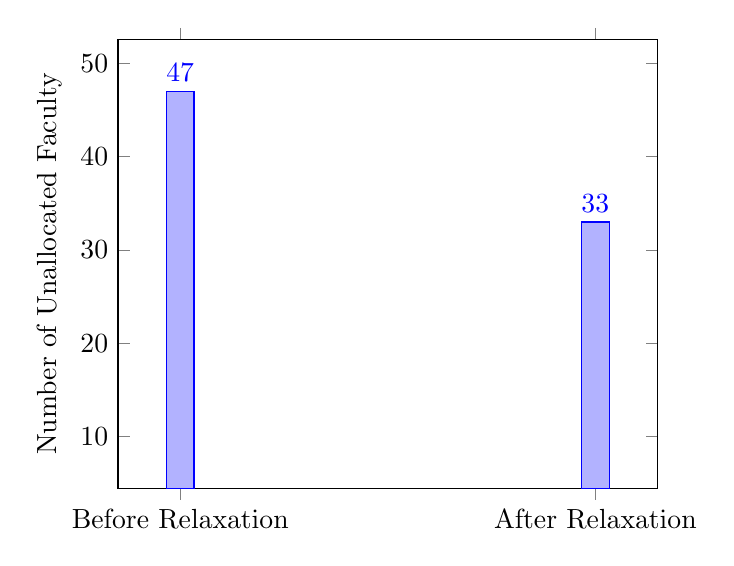
\begin{tikzpicture}

    \begin{axis}
      [
        ybar,
        ymin=10,
        enlargelimits=0.15,
        ylabel={Number of Unallocated Faculty},
        symbolic x coords={Before Relaxation, After Relaxation},
        xtick=data,
        xshift=2.5cm,
        nodes near coords,
        nodes near coords align={vertical},
      ]
      \addplot coordinates {(Before Relaxation,47) (After Relaxation,33)};

    \end{axis}
  \end{tikzpicture}
  \caption{Faculty Utilization with Workload Relaxation}
  \label{fig:faculty_utilization_workload_relaxation}
\end{figure}

\autoref{fig:faculty_utilization_workload_relaxation} shows the number of unutilized faculty members before and after workload relaxation. As visible in the figure, the number of faculty members with utilization of 0 has decreased from 47 to 33, which means that multiple faculty members were not allocated any lectures due to their workload limits being too low to accommodate any lectures at all, which is a problem also resolved by the dynamic splitting approach.

Additionally, the split of over-utilized and underutilized faculty members is 64 and 38 faculty members respectively, which points to the fact that the workload relaxation doesn't lead to a large number of faculty members being over-utilized. This is because the workload relaxation is only applied to the faculty members who are needed to teach the unallocated courses, thus only affecting a small number of faculty members.


\subsection{Dynamic Swapping Results}
\label{sec:post_allocation}

Another approach to rectify the unallocated courses is to check if there are any unallocated courses, and if, by reshuffling some of the existing allocations, faculty members can be freed up to teach the unallocated courses. This is done by finding secondary courses that are allocated to the faculty members who are needed for the unallocated courses, and checking whether these secondary courses can be allocated to other faculty members.

However, it is important to consider that the secondary courses should not be adversely impacted by this reshuffling. This means that the secondary courses should be allocated to faculty members who are nearly as suitable to teach the course as the original faculty member. This is done by checking the cost of assigning the secondary course to the other faculty members, and only reallocating the secondary course if the cost increase is within a certain threshold.

As an example, consider Course $A$, a third-year course that can be taught by a particular faculty member $F_1$. However, during the first two iterations of the allocation process for the second-year courses, $F_1$ is allocated to two other courses $B$ and $C$, exhausting their workload limits. In the pre-allocation process, we find that Course $B$ can be taught by another faculty member $F_2$ without a cost increase of 0.2, which is within the threshold of 0.5. Thus, Course $B$ is allocated to $F_2$ in the pre-allocation phase, freeing up $F_1$ to teach Course $A$.

For the pre-allocation process, we first define \autoref{alg:reassign_faculty}, which takes a faculty member and the list of their existing assignments. It then iterates over the list of existing assignments for the faculty, and checks if the lecture can be allocated to another faculty member without violating the cost threshold. If this is the case, then the lecture is allocated to the other faculty member.

\begin{algorithm}[H]
  \caption{Reassign Faculty Algorithm}
  \begin{algorithmic}[1]
    \Procedure{ReassignFaculty}{$facultyMember$, $facultyAssignments$}
    \For {$assignment \in facultyAssignments$}
    \State $lecture \gets assignment.lecture$
    \State $currentCost \gets Q(lecture, facultyMember)$
    \For {$f \in eligibleFaculty(lecture, exclude=facultyMember)$}
    \State $newCost \gets Q(lecture, f)$
    \If {$newCost - currentCost \leq costThreshold$}
    \Return $(lecture, f)$
    \EndIf
    \EndFor
    \EndFor
    \State \Return $null$
    \EndProcedure
  \end{algorithmic}
  \label{alg:reassign_faculty}
\end{algorithm}

where, $eligibleFaculty(lecture, exclude=facultyMember)$ is the list of faculty members who are eligible to teach the lecture without exceeding their workload limits, excluding the faculty member $facultyMember$.

With \autoref{alg:reassign_faculty} defined, we can define \autoref{alg:post_allocation} which takes the list of unallocated lectures and for each unallocated lecture, checks if the lecture can be allocated to another faculty member without violating the cost threshold using \autoref{alg:reassign_faculty}. If this is the case, then the lecture is allocated to the other faculty member, and the existing faculty member is allocated to the unallocated lecture.

\begin{algorithm}[H]
  \caption{Dynamic Swapping Algorithm}
  \begin{algorithmic}[1]
    \Procedure{PostAllocate}{$unallocatedLectures$, $existingAssignments$}
    \State $assignments \gets existingAssignments$
    \For {$l \in unallocatedLectures$}
    \For {$f \in eligibleFaculty(l)$}
    \State $existingLectures \gets assignments.filter(faculty=f)$
    \State $replacement \gets \text{ReassignFaculty}(f, existingLectures)$
    \If {$replacement \neq null$}
    \State $assignments \gets assignments \setminus (replacement.lecture, f)$
    \State $assignments \gets assignments \cup replacement$
    \State $assignments \gets assignments \cup (l, f)$
    \EndIf
    \EndFor
    \EndFor
    \State \Return $assignments$
    \EndProcedure
  \end{algorithmic}
  \label{alg:post_allocation}
\end{algorithm}

where $eligibleFaculty(l)$ is the list of faculty members who are eligible to teach the lecture $l$ without exceeding their workload limits.

\subsubsection{Experimental Results}

\begin{table}[H]
  \centering
  \begin{tabular}{|l|c|c|}
    \hline
    \textbf{}                 & \textbf{Before Reassignment} & \textbf{After Reassignment} \\ \hline
    \textbf{Assigned Count}   & 75                           & 78                          \\
    (Assigned Hours)          & (1214)                       & (1622)                      \\
    \textbf{Unassigned Count} & 60                           & 57                          \\
    (Unassigned Hours)        & (1392)                       & (984)                       \\
    \textbf{Allocated Hrs \%} & \textbf{46.6\%}              & \textbf{62.2\%}             \\
    \textbf{Avg Score}        & 3.61                         & 3.71                        \\
    \hline
  \end{tabular}
  \caption{Experimental Results of Dynamic Swapping}
  \label{tab:post_allocation_results}
\end{table}

\autoref{tab:post_allocation_results} shows the results of the Dynamic Swapping approach. The first column shows the results before, while the second column shows the results after the Dynamic Swapping approach is applied.

As can be seen from the results, the number of allocated lectures has increased from 75 to 78. Although a small increase in the count of allocated lectures, the percentage of allocated hours has increased from 46.6\% to 62.2\%, which is a significant improvement. This was found to be because the courses that were allocated by the Dynamic Swapping approach were large courses that had a large impact on the utilization of the faculty members.

\begin{figure}[H]
  \centering
  \resizebox{\textwidth}{!}{

    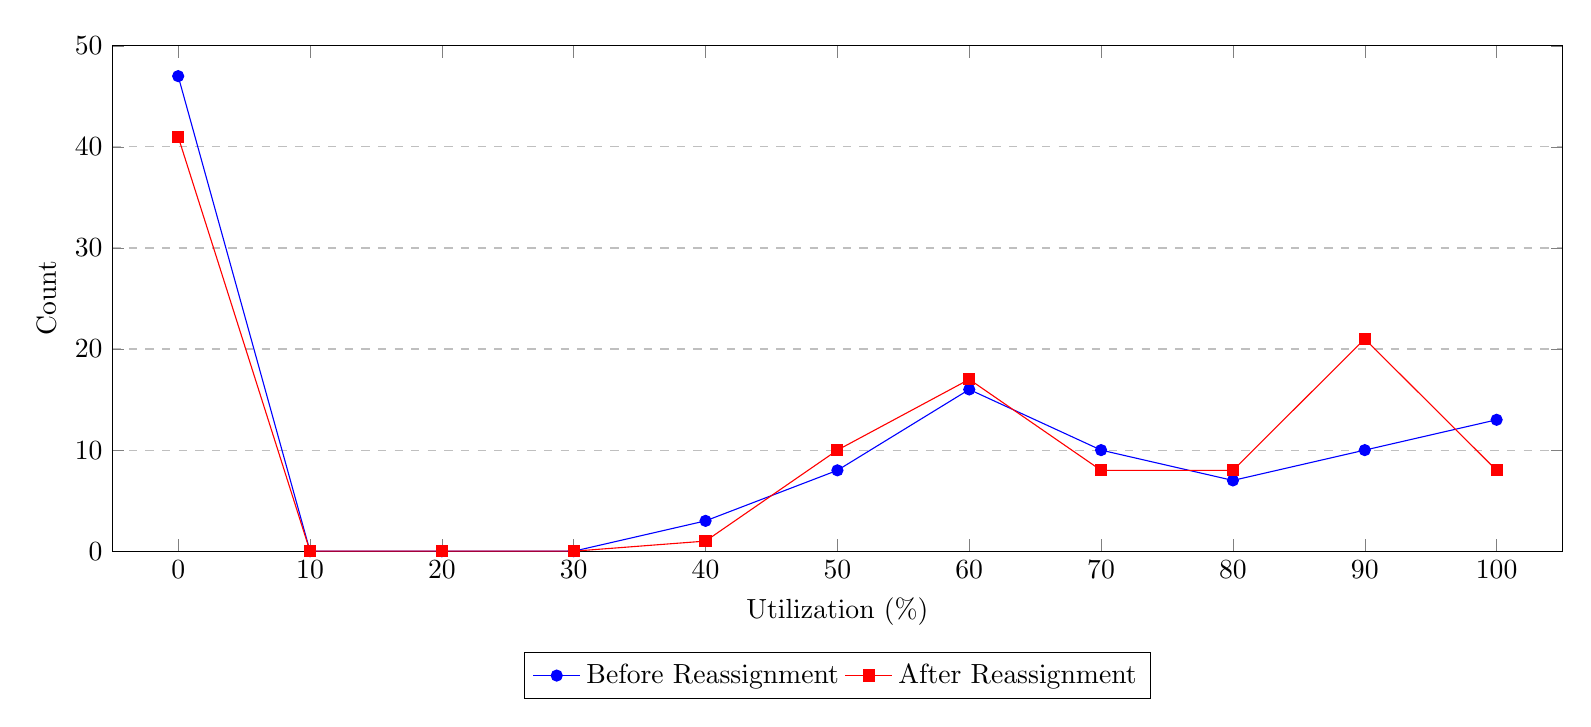
\begin{tikzpicture}
      \begin{axis}[
          xlabel={Utilization (\%)},
          ylabel={Count},
          ymin=0,
          ymax=50,
          width=20cm,
          height=8cm,
          enlarge x limits=0.05,
          legend style={at={(0.5,-0.2)},
              anchor=north,legend columns=-1},
          ymajorgrids=true,
          grid style=dashed
        ]
        \addplot[blue, mark=*] coordinates {
            (0, 47)
            (10, 0)
            (20, 0)
            (30, 0)
            (40, 3)
            (50, 8)
            (60, 16)
            (70, 10)
            (80, 7)
            (90, 10)
            (100, 13)
          };
        \addlegendentry{Before Reassignment}
        \addplot[red, mark=square*] coordinates {
            (0, 41)
            (10, 0)
            (20, 0)
            (30, 0)
            (40, 1)
            (50, 10)
            (60, 17)
            (70, 8)
            (80, 8)
            (90, 21)
            (100, 8)
          };
        \addlegendentry{After Reassignment}
      \end{axis}
    \end{tikzpicture}
  }
  \caption{Faculty Utilization with Dynamic Swapping}
  \label{fig:faculty_utilization_dynamic_swapping}
\end{figure}

\autoref{fig:faculty_utilization_dynamic_swapping} shows the utilization of faculty members with and without Dynamic Swapping processing. As visible in the figure, the number of faculty members with a utilization of 0 has decreased from 47 to 41, which means that multiple faculty members were not allocated any lectures due to their workload limits being too low to latter year courses, which were found to be too large to be allocated to some faculty members. Additionally, the overall utilization of faculty members has increased, reaching closer to optimal utilization.

\subsection{Automated Lecture Allocation Process}
\label{sec:allocation_process}

The allocation process receives the list of lectures, the list of faculty members, the student feedback scores, and the faculty preference scores as input. The lectures might already be split into multiple parts by the static splitting process defined in \autoref{sec:lecture_splitting}. Each of the lectures also has a workload associated with it, which is the number of workload units that the lecture has. This workload was defined in \autoref{ch:teaching_workload}. Additionally, it receives the relative workload limits of the faculty members as input, which are set using the approach defined in \autoref{sec:determining_equitable_teaching_workload}.

Using these inputs, the allocation process allocates the lectures to the faculty members. The allocation process is defined as follows:

\begin{enumerate}
  \item \textbf{Setup}\\
        Set the workload limits of all the faculty members using their relative workload units set in \autoref{sec:determining_equitable_teaching_workload}. Set the cost of assigning a course to a faculty member using the cost function defined in \autoref{sec:defining_the_cost_function}.
  \item \textbf{Pre-allocate}\\
        To avoid the workload limits of the faculty members being reached before all the courses are allocated, pre-allocate the courses that can be allocated immediately as defined in \autoref{sec:pre_allocation}.
  \item \textbf{Year-wise allocation}\\
        Allocate the courses with the Hungarian algorithm, using the cost matrix construction algorithm which uses the workload limits, as defined in \autoref{alg:workload_limit_cost_matrix_construction}. The lecture allocation algorithm is defined in \autoref{alg:year_wise_lec_alloc}.
  \item \textbf{Dynamic splitting}\\
        If unallocated courses remain, check if other faculty members can be allocated to the unallocated courses by splitting the courses as defined in \autoref{sec:dynamic_splitting}.
  \item \textbf{Workload limit relaxation}\\
        If unallocated courses remain, the workload limits are reached for all the faculty members. Relax the workload limits of the faculty members as defined in \autoref{sec:workload_limit_relaxation} before continuing to the next step.
  \item \textbf{Dynamic Swapping}\\
        If unallocated courses remain, check if the unallocated courses can be allocated by swapping the existing allocations, as defined in \autoref{sec:post_allocation}.
\end{enumerate}

This allocation process is summarized in \autoref{fig:allocation_process_flowchart}.

\begin{figure}[H]
  \centering
  \resizebox{\textwidth}{!}{
    \begin{tikzpicture}[node distance=0.5cm]
      \node (start) [startstop] {Start};
      \node (input) [io, below=of start] {Input: Year Lectures, Faculty, Costs, Workload Limits};
      \node (pre_alloc) [process, below=of input] {Pre Allocate Lectures};
      \node (alloc) [process, below=of pre_alloc] {Allocate Lectures Yearwise};
      \node (split_check) [decision, below=of alloc, align=center] {All Allocated?};
      \node (split) [process, right=of split_check, xshift=0.5cm] {Dynamic Splitting};
      \node (relax_check) [decision, below=of split_check, align=center] {All Allocated?};
      \node (relax) [process, right=of relax_check, xshift=0.5cm] {Relax Workload Limits};
      \node (post_check) [decision, below=of relax_check, align=center] {All Allocated?};
      \node (post_alloc) [process, right=of post_check, xshift=0.5cm] {Dynamic Swapping};
      \node (output) [io, below=of post_check] {Output: Allocated Lectures};
      \node (stop) [startstop, below=of output] {Stop};
      \draw [arrow] (start) edge (input) (input) edge (pre_alloc) (pre_alloc) edge (alloc) (alloc) edge (split_check) (split_check) edge node[anchor=south] {No} (split) (split_check) edge node[anchor=east] {Yes} (relax_check) (split) edge[out=-90, in=90] (relax_check) (relax_check) edge node[anchor=south] {No} (relax) (relax_check) edge node[anchor=east] {Yes} (post_check) (relax) edge[out=-90, in=90] (post_check) (post_check) edge node[anchor=south] {No} (post_alloc) (post_check) edge node[anchor=east] {Yes} (output) (post_alloc) edge[out=-90, in=90] (output) (output) edge (stop);
    \end{tikzpicture}
  }
  \caption{Allocation Process Flowchart}
  \label{fig:allocation_process_flowchart}
\end{figure}

\subsection{Experimental Results}

The experimental results of the allocation process are shown in \autoref{tab:overall_experimental_results}. In this process, each of the approaches defined in \autoref{sec:rectifying_unallocated_courses} are applied sequentially, incrementally improving the allocation results. The first column shows the experiment, the second column shows the number of allocated lectures as a count of lectures and the number of hours, the third column shows the number of unallocated lectures as count of lectures and the number of hours, and the fourth column shows the average score of the allocated lectures as defined by the course-faculty fit metric.

\begin{table}[H]
  \centering
  \resizebox{\textwidth}{!}{
    \begin{tabular}{|l|c|c|c|}
      \hline
      \textbf{Experiment}       & \textbf{Assigned Count (Hrs)} & \textbf{Unassigned Count (Hrs)} & \textbf{Avg Score} \\ \hline
      \textbf{Base}             & 75 (1214 hrs)                 & 60 (1392 hrs)                   & 3.61               \\ \hline
      \textbf{With Preallocate} & 84 (1640 hrs)                 & 51 (966 hrs)                    & 3.61               \\ \hline
      \textbf{Split}            & 122 (2132 hrs)                & 35 (474 hrs)                    & 3.59               \\ \hline
      \textbf{Overshoot}        & 143 (2398 hrs)                & 14 (208 hrs)                    & 3.60               \\ \hline
      \textbf{Post-Swapping}    & 154 (2540 hrs)                & 3 (66 hrs)                      & 3.60               \\ \hline
    \end{tabular}
  }
  \caption{Experimental Results}
  \label{tab:overall_experimental_results}
\end{table}

The first row shows the results of the base allocation process, which is the allocation process without any of the approaches to rectify the unallocated courses as defined in  \autoref{sec:rectifying_unallocated_courses}. As can be seen from the results, the hours of allocated lectures are 1214 hours, which is 46.6\% of the total number of hours. This is because of the greediness in the allocation process, which allocates the best faculty members to the earlier-year courses, as discussed earlier.

The second row shows the results of the same allocation process as the first row but with the pre-allocation approach used before every iteration of the Hungarian algorithm. As can be seen from the results, the number of allocated lectures has increased the number of allocated hours has increased from 1214 to 1652 hours, increasing the percentage of allocated hours from 46.6\% to 63.1\%. This is because the pre-allocation approach identifies the under-supply of faculty members and prioritizes the allocation of the courses with this under-supply, thus increasing the number of allocated hours.

The third row shows the results of the allocation process with the dynamic splitting approach used after the pre-allocation approach. As can be seen from the results, the allocated lectures have increased from 1214 hours to 2174 hours, increasing from 63.1\% to 83.2\% of the total number of hours. This is because the dynamic splitting approach breaks down the large courses that were not allocated due to the workload limits of the faculty members being reached, into smaller parts that can be allocated to the faculty members. This resulted in 18 courses being split into 2 parts, and 2 courses being split into 3 parts.

The fourth row shows the results of the allocation process with the workload relaxation approach used after the dynamic splitting approach. As can be seen from the results, the allocated lectures have increased from 2174 hours to 2398 hours, increasing from 83.2\% to 91.9\% of the total number of hours. This is because the workload relaxation approach selectively relaxes the workload limits of the faculty members who are needed to teach the unallocated courses, thus increasing the number of allocated hours.

The fifth row shows the results of the allocation process with the Dynamic Swapping approach used after the workload relaxation approach. As can be seen from the results, the allocated lectures have increased from 2398 hours to 2566 hours, increasing from 91.9\% to 98.4\% of the total number of hours. Other experiments have shown that the Dynamic Swapping approach is important for workload relaxation to be effective, since a large number of faculty members, who were previously unavailable to teach larger courses, are now available to teach these courses, thus increasing the scope for reshuffling the existing allocations.

\section{Equitable Overloading of Faculty to Resolve Unallocated Lectures}

The allocation process defined in \autoref{sec:allocation_process} allocates the courses to the faculty members in a way that doesn't overload the faculty members. This is done by setting the workload limits of the faculty members, and ensuring that the workload of the faculty members doesn't exceed their workload limits. In exceptional cases where the workload limits of the faculty members are reached and the courses cannot be allocated, the workload limits of the faculty members are relaxed as defined in \autoref{sec:workload_limit_relaxation}. This is done at the expense of bandwidth for teaching tutorials and labs for these faculty members, and in the worst case, the faculty members might be overloaded.

However, this approach is not equitable, since it leads to some faculty members being disproportionately overloaded, while not affecting the workload of other faculty members. Additionally, this approach may be suboptimal since the earlier stages of the allocation process don't account for the availability of additional workload bandwidth being available in the later stages of the allocation process. This can result in some courses being unallocated, even though they could have been allocated if the workload limits of the faculty members were relaxed.

To solve this problem, we introduce the concept of Equal Misery, which is the equitable overloading of faculty members to ensure that all the courses are allocated. The Equal Misery approach is only applied if even after the Dynamic Swapping approach, there still remain unallocated courses. This is because the Equal Misery approach may lead to more faculty members being overloaded, which is not desirable.

If the allocations are not resolved at the end of dynamic swapping, all existing allocations are discarded and the workload limits are relaxed for all the faculty members at the start of the allocation process followed by allocating the courses to the faculty members using the same process as defined in \autoref{sec:allocation_process}. If the workload limits of the faculty members are still reached, then the workload limits of the faculty members are relaxed again by a marginal amount to accommodate the outlying courses.

Thus, the overall approach can be revised as shown in \autoref{fig:allocation_process_flowchart_equal_misery}.

\begin{figure}[H]
  \centering
  \resizebox{\textwidth}{!}{
    \begin{tikzpicture}[node distance=0.5cm]
      \node (start) [startstop] {Start};
      \node (input) [io, below=of start] {Input: Year Lectures, Faculty, Costs, Workload Limits};
      \node (alloc_process) [process, below=of input] {Allocate Lectures};
      \node (equal_misery_check) [decision, below=of alloc_process, align=center] {All Allocated?};
      \node (discard_alloc) [process, right=of equal_misery_check, xshift=0.5cm] {Discard Existing Allocations};
      \node (relax) [process, below=of discard_alloc] {Relax Workload Limits};
      \node (rerun_alloc) [process, below=of relax] {Rerun Allocation};
      \node (output) [io, below=of equal_misery_check, yshift=-4cm] {Output: Allocated Lectures};
      \node (stop) [startstop, below=of output] {Stop};
      \draw [arrow] (start) edge (input) (input) edge (alloc_process) (alloc_process) edge (equal_misery_check) (equal_misery_check) edge node[anchor=south] {No} (discard_alloc) (discard_alloc) edge (relax) (relax) edge (rerun_alloc) (rerun_alloc) edge[out=-90, in=90] (output) (equal_misery_check) edge node[anchor=east] {Yes} (output) (output) edge (stop);
      \node[draw=red,dotted,fit=(discard_alloc) (relax) (rerun_alloc), inner sep=0.3cm, label={[red]Equal Misery Approach}, rounded corners] {};
    \end{tikzpicture}
  }
  \caption{Allocation Process Flowchart with Equal Misery}
  \label{fig:allocation_process_flowchart_equal_misery}
\end{figure}

\subsection{Experimental Results}


\begin{table}[H]
  \centering
  \resizebox{\textwidth}{!}{
    \begin{tabular}{|l|c|c|c|}
      \hline
      \textbf{Experiment}       & \textbf{Assigned Count (Hrs)} & \textbf{Unassigned Count (Hrs)} & \textbf{Avg Score} \\ \hline
      \textbf{With Preallocate} & 122 (2370)                    & 13 (236)                        & 3.65               \\ \hline
      \textbf{Split}            & 129 (2456)                    & 10 (150)                        & 3.65               \\ \hline
      \textbf{Overshoot}        & 131 (2480)                    & 8 (126)                         & 3.64               \\ \hline
      \textbf{Dynamic Swapping} & 137 (2591)                    & 2 (15)                          & 3.66               \\ \hline
    \end{tabular}
  }
  \caption{Experimental Results of Equal Misery}
  \label{tab:equal_misery_results}
\end{table}

\autoref{tab:equal_misery_results} shows the results of the allocation process with the Equal Misery approach. As can be seen from the results, the unassigned lectures are much lower at every stage of the process. This is because the Equal Misery approach relaxes the workload limits of the faculty members, thus increasing the bandwidth of the faculty members to teach courses. This results in more courses being allocated at every stage of the process.

Another notable insight from the results is that the average score of the allocated lectures is higher than the average score of the allocated lectures in the base allocation process. This is because, with the Equal Misery approach, the workload limits of the faculty members are relaxed, thus increasing the bandwidth of high-performing faculty members to teach more courses as well, thus increasing the average score of the allocated lectures.

It is important to note that for the dataset used in this thesis, the Equal Misery approach led to only marginal improvements in the allocation results. However, this approach is important to consider, since it ensures that the workload of the faculty members is distributed equally, and no faculty member is disproportionately overloaded.

\section{Summary}

In this chapter, we defined the various priorities that decide which faculty is suited to teach which course. We then defined the allocation problem and all of the constraints and objectives that it aims to optimize. Using this, we modeled the allocation process and used the Hungarian Algorithm to solve the allocation problem. We further refined the allocation process, adding a mechanism to honor the workload limits and a mechanism to handle the management priority of allocating earlier-year courses to the best faculty, before defining the cost function which represents the priorities of the students and the faculty.

We found various shortcomings in the allocation process which resulted in unallocated lectures. We then defined various approaches to rectify these shortcomings. These included the pre-allocation approach which prioritizes the allocation of courses with an under-supply of faculty members, the dynamic splitting approach which splits the courses that are not allocated due to the workload limits of the faculty members being reached, the workload relaxation approach which relaxes the workload limits of the faculty members to accommodate the unallocated courses, and the Dynamic Swapping approach which reshuffles the existing allocations to accommodate the unallocated courses.

We implemented these approaches as part of the allocation process and found that the allocation process with all of these approaches was able to allocate 98.4\% of the total number of hours, a substantial increase from the 46.6\% of the total number of hours allocated by the allocation process originally. We also found that the Equal Misery approach, which equitably overloads the faculty members to ensure that all the courses are allocated, was able to allocate 98.4\% of the total number of hours as well, with the average score of the allocated lectures being higher than the average score of the allocated lectures in the base allocation process.

In the next chapter, we will discuss the implementation of the allocation process for tutorial and lab allocation, which is a similar problem to the lecture allocation problem, but with a few key differences. We will discuss ways to adapt the allocation process to the tutorial and lab allocation problem, and the results of the implementation of the allocation process for tutorial and lab allocation.
